\chapter{Demonstração}

De seguida, iremos ver uma demonstração das capacidades do \textit{middleware}, fazendo uso da aplicação cliente e dos simuladores de dispositivos, desenvolvidos para este efeito. Neste capítulo vamos detalhar o ambiente utilizado para a demonstração, assim como todas as funcionalidades chave do \textit{middleware}, desde a configuração inicial de um \textit{hub} até à definição de tarefas automatizadas.

\section{Preparação}

Para efetuar esta demonstração instalou-se o \textit{hub} num \textit{Raspberry PI} a correr o sistema operativo \textit{Raspbian}, basicamente uma versão para processadores ARM do popular sistema operativo baseado em \textit{Linux}, \textit{Debian}. Além disto teremos 3 simuladores de dispositivos a correr neste sistema, uma fechadura, um sensor de movimento e um termostato.

Num cenário real, um utilizador teria uma \textit{box} já pré-configurada que continha o \textit{software} respetivo ao \textit{hub}, e alguns dispositivos já instalados na sua residência. Neste caso, todos os dispositivos correm a partir do mesmo \textit{Raspberry} assim como o \textit{hub}, apenas para efeitos de demonstração, o funcionamento seria o mesmo caso eles estivessem a ser simulados noutros sistemas.

A aplicação será testada no modo de desenvolvimento, ou seja, a aplicação corre num \textit{browser} num \textit{desktop} de desenvolvimento em vez de um dispositivo \textit{mobile}, isto porque é mais prático para efeitos de testes e documentação desta demonstração. Apesar disto, a aplicação foi testada no sistema operativo \textit{Android}, e retinha toda a funcionalidade demonstrado no modo de desenvolvimento.

Além disto, também fizemos uso do emulador do \textit{Philips Hue}\footnote{\url{http://steveyo.github.io/Hue-Emulator/}}, a correr no sistema de desenvolvimento onde se vai testar a aplicação. 

De seguida poderemos ver a distribuição destes componentes na Figura \ref{fig:demo-setup}.

\begin{figure}[H]
  \centering
        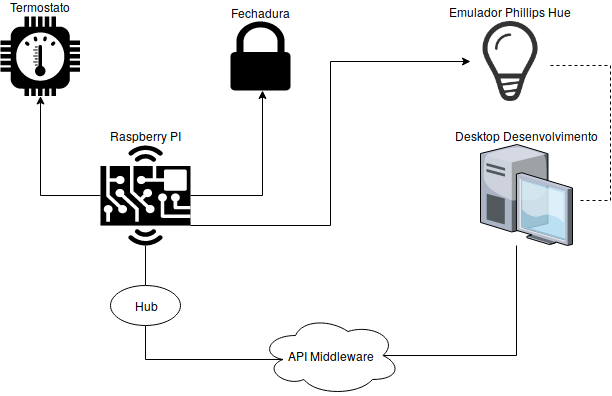
\includegraphics[scale=0.6]{img/demo/setup.png}
  \caption{Componentes preparados para a demonstração}
  \label{fig:demo-setup}
\end{figure}

De notar que apesar da própria aplicação cliente estar a correr na mesma rede local dos dispositivos e do \textit{hub}, toda a comunicação é feita através da API do \textit{middleware}, recorrendo ao software de \textit{tunneling} que já descrevemos anteriormente.

\section{Execução}

Agora vamos então efetuar a demonstração prática do \textit{middleware}, recorrendo à aplicação cliente. Primeiro iremos verificar o registo e o \textit{login} de um utilizador, seguido depois da configuração do seu espaço casa e do seu \textit{hub}, passando depois pela configuração de alguns dispositivos, finalizando com a criação de um cenário e de algumas tarefas automatizadas.

Inicialmente temos, como é costume, o ecrã inicial de \textit{login}, com uma opção para criar um utilizador.

\begin{figure}[H]
  \centering
        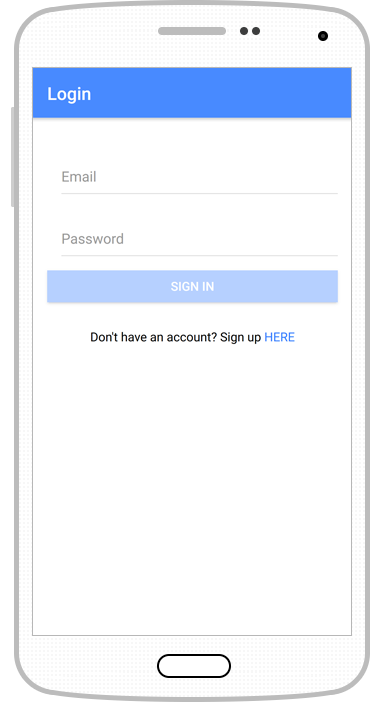
\includegraphics[scale=0.6]{img/demo/login.png}
  \caption{Ecrãs de demonstração: \textit{Login}}
\end{figure}

Como não possuímos nenhum utilizador, deveremos efetuar o registo.

\begin{figure}[H]
  \centering
        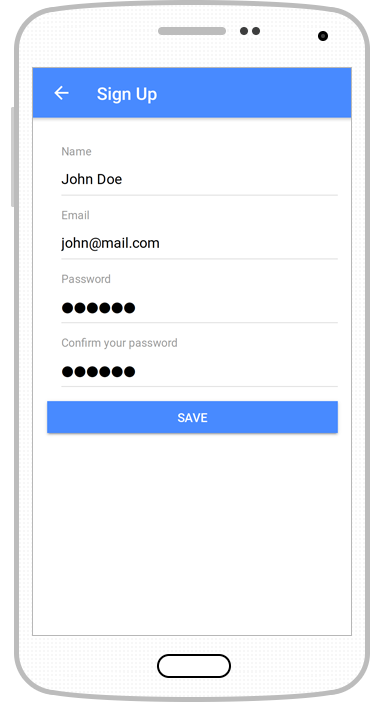
\includegraphics[scale=0.6]{img/demo/register.png}
  \caption{Ecrãs de demonstração: Registo}
\end{figure}

Após o registo ficamos perante o ecrã base da aplicação, neste caso com um aviso para o utilizador criar a sua primeira casa. 

\begin{figure}[H]
  \centering
        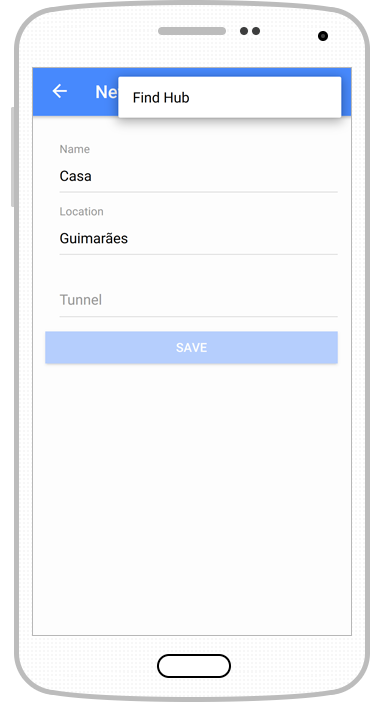
\includegraphics[scale=0.6]{img/demo/create_home.png}
  \caption{Ecrãs de demonstração: Criar casa}
\end{figure}

Para criar uma casa necessitamos do URL do \textit{hub}, que pode ser descoberto com a ferramenta \textit{''Find Hub''}. Este mecanismo já foi explicitado anteriormente, na detalhação do mecanismo de \textit{tunneling}. Aqui simplesmente extraímos o \textit{tunel} disponibilizado pelo \textit{hub}.

\begin{figure}[H]
  \centering
        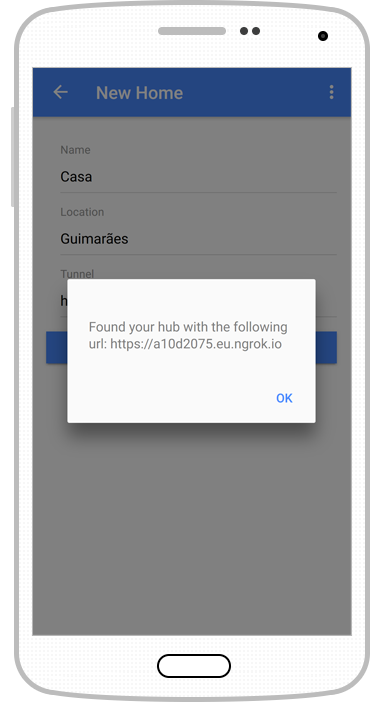
\includegraphics[scale=0.6]{img/demo/create_home_find_hub.png}
  \caption{Ecrãs de demonstração: Descoberta do \textit{hub}}
\end{figure}

Depois o nosso ecrã inicial mostra as casas do utilizador, uma vez que o \textit{middleware} suporta várias casas, por exemplo, caso o utilizador tivesse uma casa de férias poderia colocá-la aqui também.

\begin{figure}[H]
  \centering
        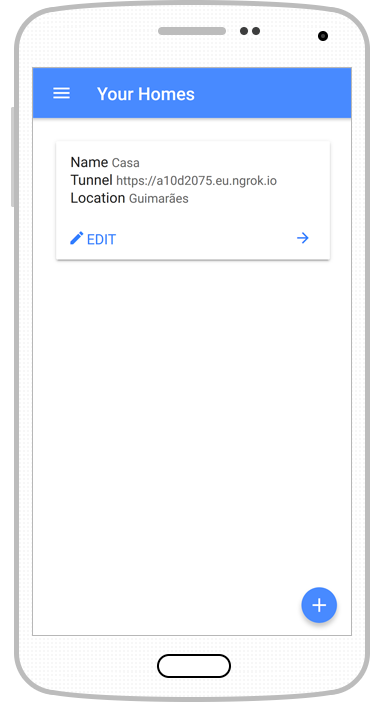
\includegraphics[scale=0.6]{img/demo/list_home.png}
  \caption{Ecrãs de demonstração: Lista de Casas}
\end{figure}

Clicando na casa que acabou de ser criada, ficamos perante o ecrã base da casa, possuindo 3 separadores, \textit{scenarios}, \textit{things} e \textit{tasks}. Por omissão, somos redirecionados para o separador \textit{things}, onde podemos gerir os dispositivos que um utilizador tem.

\begin{figure}[H]
  \centering
        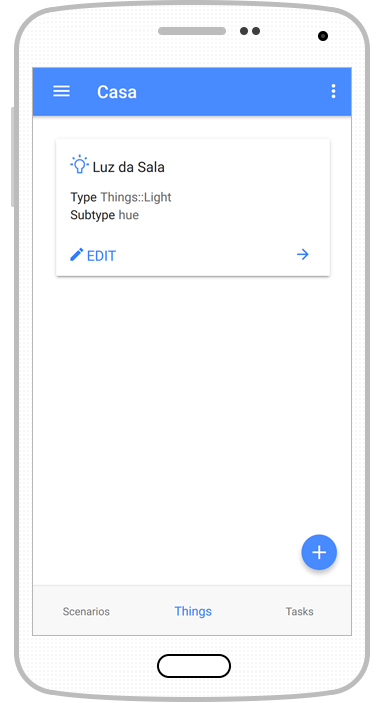
\includegraphics[scale=0.6]{img/demo/list_things.png}
  \caption{Ecrãs de demonstração: Lista de Dispositivos}
\end{figure}

De momento não possuímos qualquer tipo de dispositivo configurado, portanto vamos então iniciar esse processo carregando no ícone de adição, no canto inferior direito do ecrã. O objetivo irá passar por configurar uma lâmpada do emulador do \textit{Philips Hue}, recorrendo ao serviço de descoberta.

\begin{figure}[H]
  \centering
        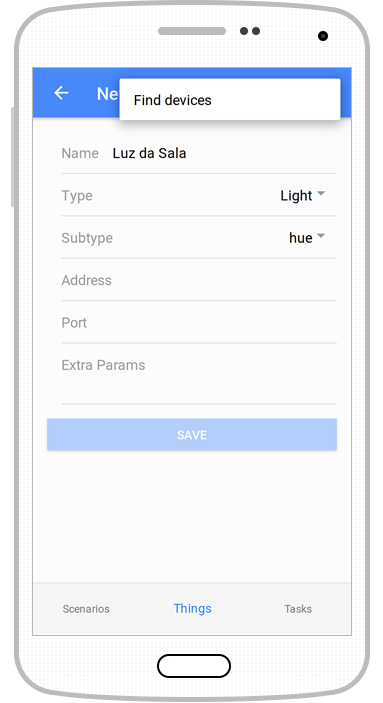
\includegraphics[scale=0.6]{img/demo/new_thing.png}
  \caption{Ecrãs de demonstração: Criar Dispositivo}
\end{figure}

Neste ecrã da Figura 24, preenchemos os parâmetros de conexão ao dispositivo, deixando o endereço por preencher, uma vez que iremos recorrer ao serviço de descoberta do \textit{hub} para o localizar. O serviço de descoberta irá preencher os campos necessários, sendo depois necessário preencher os \textit{extra params} com o ID da lâmpada. Aqui conseguimos observar a modularidade do \textit{middleware}, onde cada subtipo possui o seu próprio subconjunto de parâmetros de configuração, sendo possível associar com qualquer tipo de dispositivo desde que haja um serviço para o mesmo. Neste caso o \textit{extra params} é apenas um \textit{input} de JSON, não sendo ótimo em termos de usabilidade, servindo apenas para efeitos de demonstração. Num cenário ideal, cada subtipo teria um formulário diferente com os parâmetros necessários ao seu funcionamento.

\begin{figure}[H]
  \centering
        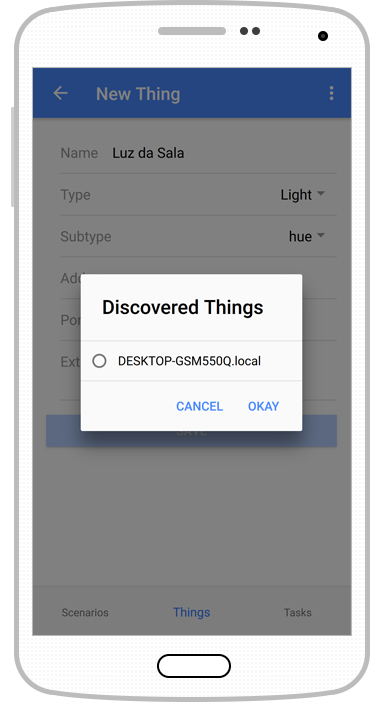
\includegraphics[scale=0.6]{img/demo/new_thing_discovery.png}
  \caption{Ecrãs de demonstração: Descoberta de Dispositivo}
\end{figure}

Depois de executar o serviço de descoberta ficamos com o endereço do dispositivo, podendo assim gravar a configuração e ganhar acesso aos controlos do mesmo. Nos \textit{extra params} inserimos o \textit{light\_id} da nossa lâmpada, normalmente é possível obter este ID através da aplicação oficial do \textit{Phillips Hue}, no nosso caso o ID é obtido dentro do emulador.

\begin{figure}[H]
  \centering
        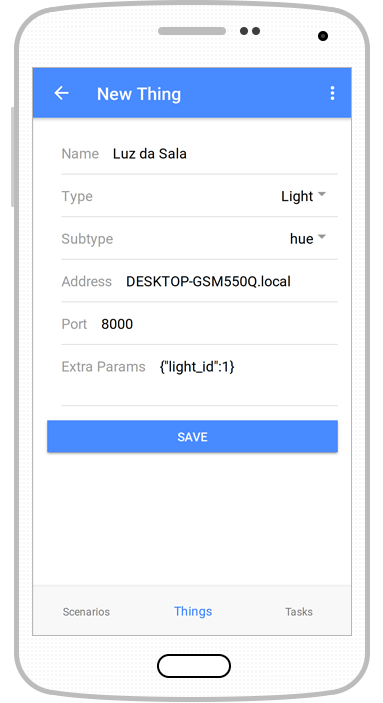
\includegraphics[scale=0.6]{img/demo/new_things_full.png}
  \caption{Ecrãs de demonstração: Descoberta de Dispositivo}
\end{figure}

De seguida podemos ver então o ecrã da lista de dispositivos já atualizado, assim como o ecrã base das informação e controlos de um dispositivo, onde podemos interagir com o mesmo.

\begin{figure}[H]
  \centering
        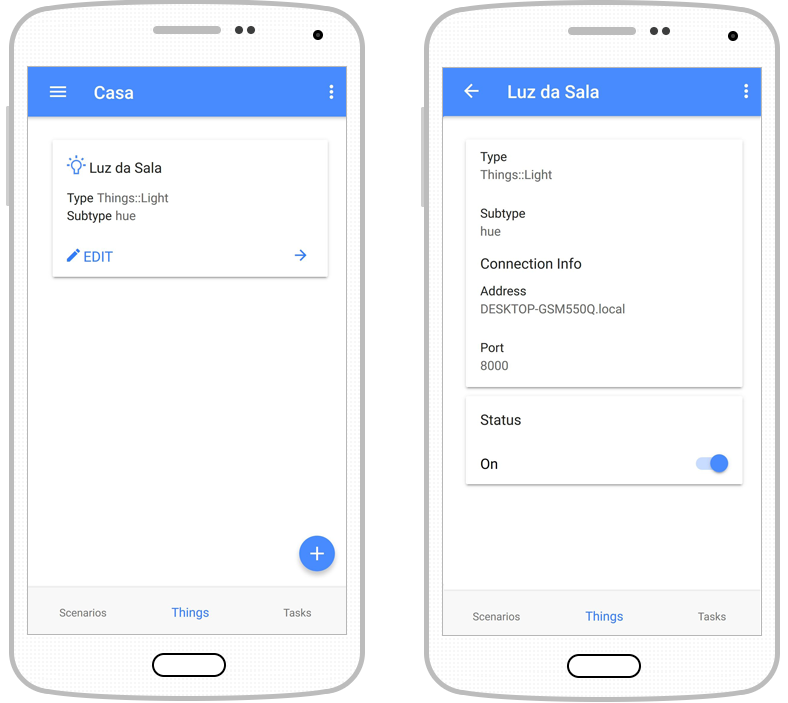
\includegraphics[scale=0.4]{img/demo/new_things_list_info.png}
  \caption{Ecrãs de demonstração: Lista de Dispositivos}
\end{figure}

Neste ecrã da direita podemos desligar ou ligar a luz, tendo um \textit{feedback} real, ou seja, se por alguma razão a luz não acender a aplicação é notificada (ativação síncrona). Se a luz for desligada por outra aplicação também nos apercebemos disso, uma vez que este ecrã está ligado ao \textit{middleware} através de \textit{websockets}, recebendo atualizações em tempo real do estado do dispositivo.

Para esta demonstração configuramos mais 3 dispositivos, uma fechadura/porta, um termostato e um sensor de movimento, seguindo o mesmo método que foi mostrado anteriormente. Agora vamos mostrar as funcionalidades mais avançadas, nomeadamente os cenários e as tarefas.

No menu cenários podemos criar um cenário com um nome, um processo muito simples, e depois disto podemos então adicionar dispositivos e o seu estado desejado ao cenário. 

\begin{figure}[H]
  \centering
        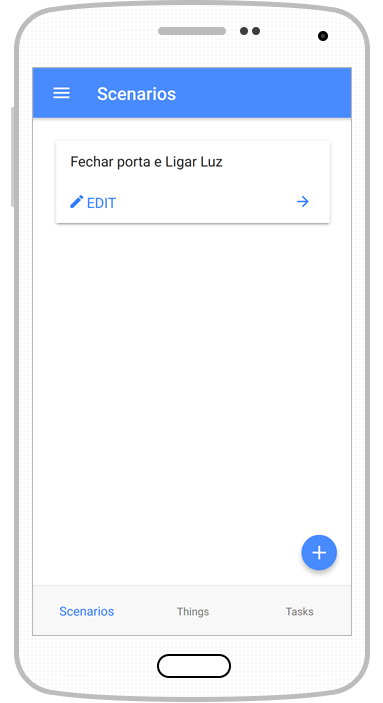
\includegraphics[scale=0.6]{img/demo/list_scenario.png}
  \caption{Ecrãs de demonstração: Ecrã de Cenário}
\end{figure}

De momento é impossível aplicar o cenário, dado que o mesmo não tem nenhum dispositivo associado, portanto para fazer jus ao nome do mesmo, iremos adicionar um dispositivo ''porta'' com a ação ''fechar'' e um dispositivo ''luz'' com a ação ''ligar''.

\begin{figure}[H]
  \centering
        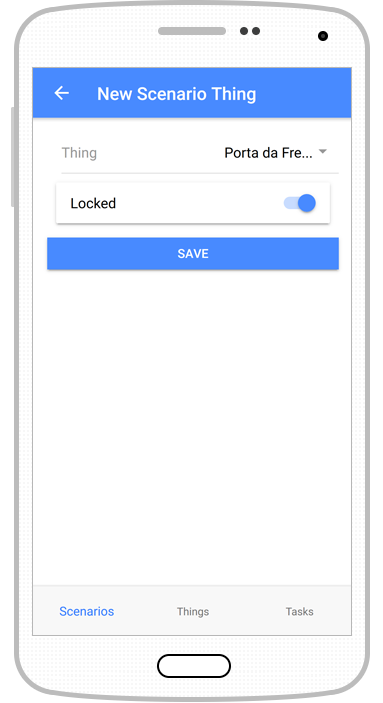
\includegraphics[scale=0.6]{img/demo/new_scenario_thing_lock.png}
  \caption{Ecrãs de demonstração: Criação de um \textit{Scenario Thing}}
\end{figure}

Acima podemos ver o ecrã para adicionar \textit{scenario things}, neste caso a adicionar a ação ''fechar porta'' ao cenário em questão.

\begin{figure}[H]
  \centering
        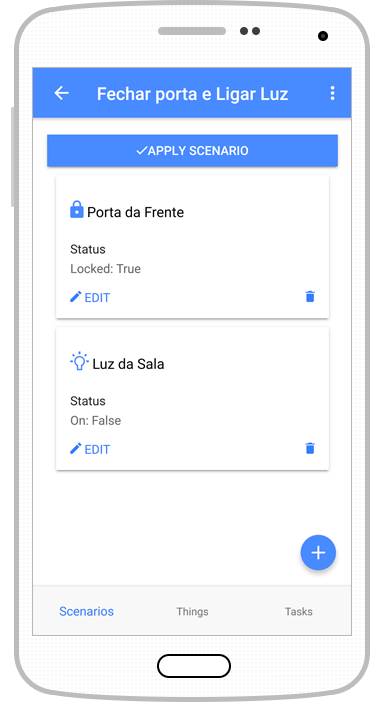
\includegraphics[scale=0.6]{img/demo/show_scenario_with_things.png}
  \caption{Ecrãs de demonstração: Ecrã de Cenário válido}
\end{figure}

Como podemos ver temos então as duas ações que desejávamos, podendo aplicá-las aos dispositivos em questão. Ao clicar naquele botão vamos interagir com o tal recurso \textit{Scenario Applier}, como já vimos na arquitetura, que irá delegar ao \textit{DelayedJob} a ativação dos dispositivos em série. A aplicação não recebe a confirmação da ativação dos mesmos como no caso do ecrã singular de um dispositivo. De seguida poderemos ver os \textit{logs} do simulador, de notar que o primeiro corresponde ao nosso simulador enquanto que o segundo corresponde ao emulador do \textit{Philips Hue}, sendo que o primeiro possui o \textit{timestamp} em UTC e o segundo na hora do sistema (\textit{timezone} de Lisboa).

\begin{figure}[H]
  \centering
        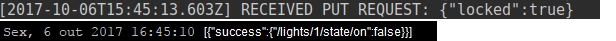
\includegraphics[scale=0.6]{img/demo/scenario_apply_log.jpg}
  \caption{Ecrãs de demonstração: \textit{Log} de aplicação de cenário}
\end{figure}

Por fim iremos abordar o separador das \textit{tasks}, que inclui as funcionalidades das \textit{timed} e \textit{triggered} \textit{tasks}. Como já vimos anteriormente, uma tarefa pode aplicar um cenário ou um único dispositivo com base num dado contexto, uma expressão \textit{cron} ou o estado de um outro dispositivo.

Primeiramente iremos ver como se configura uma \textit{timed task}. De notar a opção entre a escolha de um cenário ou um dispositivo como alvo, neste caso iremos escolher um dispositivo. A expressão \textit{cron} irá ativar esta tarefa precisamente as 16:00, todos os dias, no \textit{timezone} \textit{Europe/Lisbon} (este último aspeto das expressões \textit{cron} é exclusivo ao \textit{DelayedCronJob}). 

\begin{figure}[H]
  \centering
        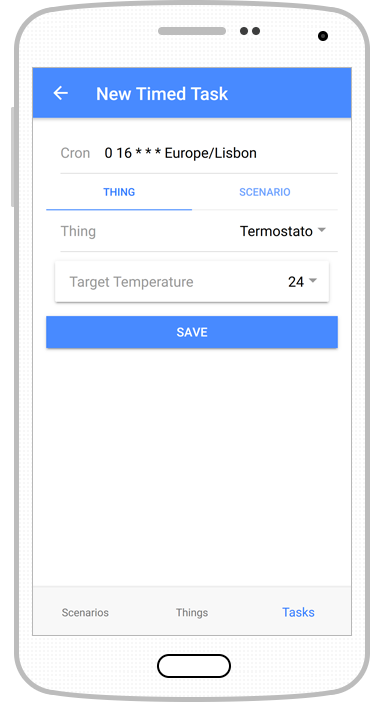
\includegraphics[scale=0.6]{img/demo/new_timed_task.png}
  \caption{Ecrãs de demonstração: Criar \textit{Timed Task}}
\end{figure}

Depois de criada a tarefa podemos ver o campo \textit{Next Run} a mostrar a próxima execução da tarefa. Isto irá definir a temperatura do termostato a 24ºC às 16:00.

\begin{figure}[H]
  \centering
        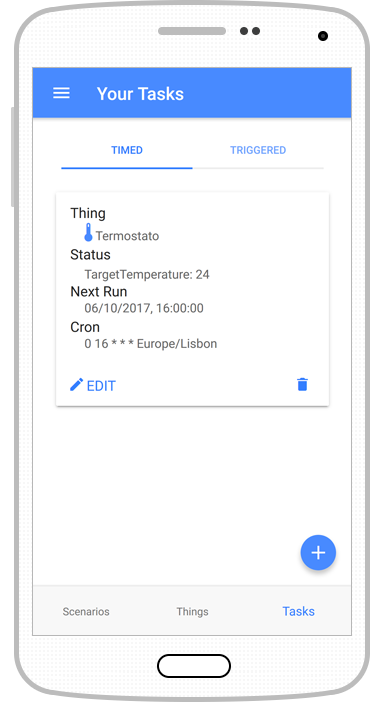
\includegraphics[scale=0.6]{img/demo/show_timed_task.png}
  \caption{Ecrãs de demonstração: Lista \textit{Timed Tasks}}
\end{figure}

Para comprovar o funcionamento deste mecanismo, podemos observar os \textit{logs} do simulador (tempo UTC), que recebe um pedido para alterar o estado segundos após as 16:00.

\begin{figure}[H]
  \centering
        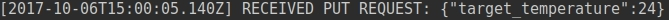
\includegraphics[scale=0.6]{img/demo/timed_task_log.jpg}
  \caption{Ecrãs de demonstração: Logs {Timed Task}}
\end{figure}

Para concluir a demonstração, um exemplo de \textit{triggered tasks}. Aqui vamos criar uma tarefa que ao detetar movimento num sensor irá ativar o cenário previamente definido, ''fechar porta e ligar luz''. 

\begin{figure}[H]
  \centering
        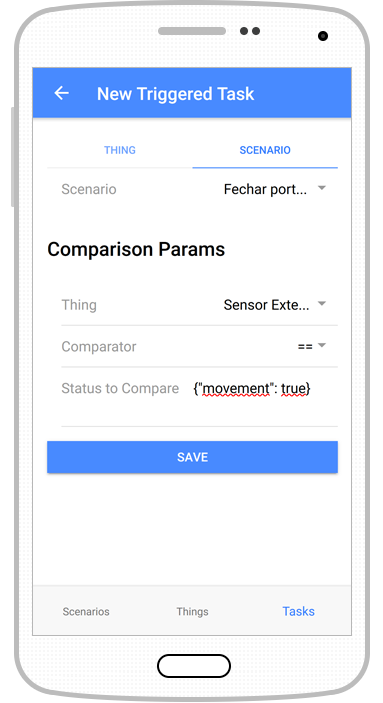
\includegraphics[scale=0.6]{img/demo/new_triggered_task.png}
  \caption{Ecrãs de demonstração: Criar \textit{Triggered Task}}
\end{figure}

Tal como o campo \textit{extra params}, o campo \textit{status to compare} também é um campo textual em formato JSON, útil para demonstração mas mau em termos de usabilidade. Num cenário ideal o utilizador escolheria os valores que queria comparar e utilizava inputs adequados para o efeito. Mesmo assim, a combinação entre o comparador e o estado traduz-se para a ação ''movimento detetado no sensor'', alcançando o nosso objetivo.

\begin{figure}[H]
  \centering
        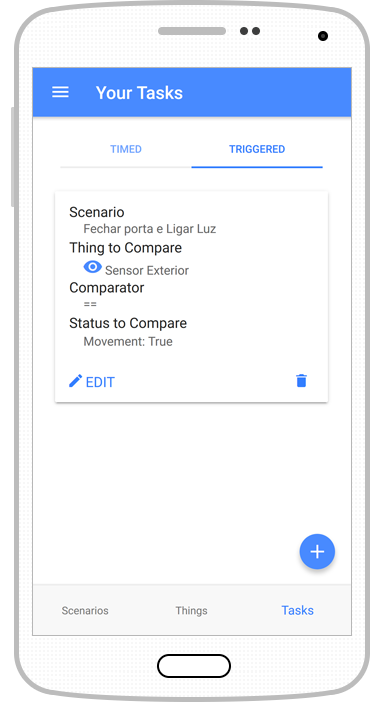
\includegraphics[scale=0.6]{img/demo/show_triggered_task.png}
  \caption{Ecrãs de demonstração: Lista \textit{Triggered Tasks}}
\end{figure}

O sensor de movimento tem que ser ativado manualmente, através do simulador, e depois disto iremos visualizar os \textit{logs} de ambos os dispositivos associados ao cenário para verificar a ativação dos mesmos, de modo a comprovar o funcionamento deste mecanismo.

\begin{figure}[H]
  \centering
        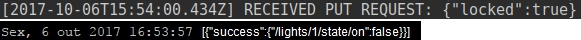
\includegraphics[scale=0.6]{img/demo/logs_triggered_task.jpg}
  \caption{Ecrãs de demonstração: Logs \textit{Triggered Task}}
\end{figure}

Como podemos ver, ambos os dispositivos são ativados com uma diferença de segundos entre os mesmos, comprovando o funcionamento das \textit{triggered tasks}.

Para concluir, toda esta demonstração mostrou as funcionalidades do \textit{middleware}, com algumas provas concretas mostradas através dos \textit{logs}. Mesmo assim, além deste teste ''manual'', todos os módulos da aplicação possuem testes unitários, sendo que estes testes ''manuais'' apenas têm como função analisar a interação entre os diversos módulos do sistema, o \textit{hub}, os dispositivos e o \textit{middleware}.